% nt-02-existentialism.tex

\documentclass[xcolor=dvipsnames]{beamer}
\usepackage{teachbeamer}

\title{Existentialism}
\subtitle{{\CourseNumber}, {\CourseInst}}

\author{\CourseName}

\date{May 22, 2018}

\begin{document}

\begin{frame}
  \titlepage
\end{frame}

% \begin{frame}
%   \frametitle{iClicker Question}
% Choose from the following options. This item will be graded.
% \begin{block}{iClicker Question}
% [4724] What is the cornerstone of existentialism?
% \end{block}
% \begin{description}
% \item[A\hspace{.2in}$\blacktriangleright$] man is not free but bound to his existence
% \item[B\hspace{.2in}$\blacktriangleright$] man's existence is more firmly established than God's existence
% \item[C\hspace{.2in}$\blacktriangleright$] everything is morally permissible
% \item[D\hspace{.2in}$\blacktriangleright$] existence precedes essence
% \end{description}
% \end{frame}

% \begin{frame}
%   \frametitle{iClicker Question}
% Choose from the following options. This item will be graded.
% \begin{block}{iClicker Question}
% [1387] Which of these are not part of a Sartre illustration in his paper?
% \end{block}
% \begin{description}
% \item[A\hspace{.2in}$\blacktriangleright$] the picture of Dorian Gray
% \item[B\hspace{.2in}$\blacktriangleright$] joining the resistance or staying with one's mother
% \item[C\hspace{.2in}$\blacktriangleright$] joining a Christian or a Communist trade union
% \item[D\hspace{.2in}$\blacktriangleright$] a man who becomes a Jesuit after many setbacks in life
% \end{description}
% \end{frame}

% \begin{frame}
%   \frametitle{iClicker Question}
% Choose from the following options. This item will be graded.
% \begin{block}{iClicker Question}
% [4435] Which one of these is a core moral dilemma in Charles Taylor's essay
% ``What Is Human Agency?''?
% \end{block}
% \begin{description}
% \item[A\hspace{.2in}$\blacktriangleright$] legalizing abortion vs valuing human life
% \item[B\hspace{.2in}$\blacktriangleright$] keeping one healthy person alive vs having five sick patients die
% \item[C\hspace{.2in}$\blacktriangleright$] persisting in an academic job vs moving to Nepal
% \item[D\hspace{.2in}$\blacktriangleright$] eating organic local food vs giving to charity
% \end{description}
% \end{frame}

% \begin{frame}
%   \frametitle{iClicker Question}
% Choose from the following options. This item will be graded.
% \begin{block}{iClicker Question}
% [3878] Which of these contrast pairs is not a distinction found in Charles
% Taylor's paper?
% \end{block}
% \begin{description}
% \item[A\hspace{.2in}$\blacktriangleright$] qualitative and quantitative evaluation
% \item[B\hspace{.2in}$\blacktriangleright$] weak and strong evaluation
% \item[C\hspace{.2in}$\blacktriangleright$] first and second order desires
% \item[D\hspace{.2in}$\blacktriangleright$] internalist and externalist evaluation
% \end{description}
% \end{frame}

% \begin{frame}
%   \frametitle{iClicker Question}
% Choose from the following options. This item will be graded.
% \begin{block}{iClicker Question}
% [1203] Which of these characters appear as examples in Alexander
% Nehamas chapter ``How One Becomes What One Is''?
% \end{block}
% \begin{description}
% \item[A\hspace{.2in}$\blacktriangleright$] Ulysses (Joyce), Ahab (Melville), Anna Karenina (Tolstoy)
% \item[B\hspace{.2in}$\blacktriangleright$] Gregor Samsa (Kafka), Elizabeth Bennet (Austen), Gatsby (Fitzgerald)
% \item[C\hspace{.2in}$\blacktriangleright$] Hamlet (Shakespeare), Jeremiah (Hebrew Bible), Vergil (Dante)
% \item[D\hspace{.2in}$\blacktriangleright$] Charlus (Proust), Odysseus (Homer), Zarathustra (Nietzsche)
% \end{description}
% \end{frame}

% \begin{frame}
%   \frametitle{iClicker Question}
% Choose from the following options. This item will be graded.
% \begin{block}{iClicker Question}
% [1997] What, according to Nehamas, characterizes the unity of a life
% in Nietzsche?
% \end{block}
% \begin{description}
% \item[A\hspace{.2in}$\blacktriangleright$] a metaphysical soul
% \item[B\hspace{.2in}$\blacktriangleright$] social acceptance as a subject
% \item[C\hspace{.2in}$\blacktriangleright$] organization and coherence
% \item[D\hspace{.2in}$\blacktriangleright$] a life-time unifying narrative
% \end{description}
% \end{frame}

\begin{frame}
  \frametitle{What the Self Is Not}
  Nehamas contrasts Nietzsche's view of the self with the following.
  \begin{description}
  \item[Descartes] an immortal and indivisible subject existing
    separately from the body
  \item[Descartes (again)] the source of thought
  \item[Freud] the core whose appearance is consciousness
  \item[Parfit/Carruthers] a Humean collection whose unity is
    secondary
  \item[Plato] a tripartite organism of appetites, spirit, and mind,
    over whom the mind should rule
  \item[Aristotle] a lifetime with narrative/moral coherence
  \end{description}
\end{frame}

\begin{frame}
  \frametitle{Becoming What One Is}
  There are several interpretive problems with ``becoming what one
  is.'' How are they resolved?
  \begin{enumerate}
  \item what does Nietzsche mean by ``what one is,'' when he considers
    the self by and large a malignant invention?
  \item what does it mean to call upon someone to ``become what one
    is'' when there is no such thing as free will?
  \item what is the underlying unity of that which one is, if it is
    neither physiological nor psychological nor metaphysical?
  \end{enumerate}
\end{frame}

\begin{frame}
  \frametitle{Recommendations}
  According to Nehamas, Nietzsche has the following recommendations to
  become what one is.
  \begin{itemize}
  \item human beings with a strong will create their own laws (they are new, unique, incomparable)
  \item they allow for organization and coherence (they do not
    entertain tolerance towards themselves)
  \item they prefer brief habits to the development of character
    (contra Aristotle), knowing that the future threatens any unity
    found between the present and the past
  \item they affirm eternal recurrence  \end{itemize}
\end{frame}

\begin{frame}
  \frametitle{Reproaches Against Existentialism}
  \begin{itemize}
  \item quietism (communists) intellectual contemplation leads to just
    another bourgeois worldview
  \item privileging the solitary over solidarity, forgetting the
    ``smile of the infant'' (Catholics)
  \item the seriousness of human affairs and moral responsibility (Christians)
  \end{itemize}
  JPS: They call us gloomy, when they say (dismal proverbs), ``charity
  begins at home''
\end{frame}

\begin{frame}
  \frametitle{Existence Precedes Essence}
  In the 18th century, the idea of the artisan-designer for human
  beings was sidelined, but the quest for a human essence remained.
  The paper knife.
  \begin{itemize}
  \item ``man surges up in the world and defines himself afterwards''
  \item man differs from a scientific object because he is nothing
    until he makes something of himself
  \item in choosing for himself he chooses for all men (Christian
    trade union, monogamy)
  \item man is condemned to be free
  \end{itemize}
\end{frame}

\begin{frame}
  \frametitle{Open Questions}
  \begin{itemize}
  \item How typical is the Free French example for a moral dilemma?
  \item Man fashions both the signs and their interpretation
    $\longrightarrow$ the importance of hermeneutics for ethics
    (Jesuit priest)
  \item Sartre's reliance on Kant (``one ought always to ask oneself
    what would happen if everyone did as one is doing,'' 292) and
    Descartes (``the starting point for truth is one's immediate sense
    of self'', 302)
  \item Contrast human nature with the human condition to understand
    what Sartre means by cowardice. ``Those who hide from total
    freedom, in a guise of solemnity or with deterministic excuses, I
    shall call cowards'' (308). The story of Carlos Flores and the
    subway accident.
  \item How appropriate is it to demand strict authenticity from
    humans? Don't we need an essence for authenticity, for ``being who
    we are''? Michel Foucault's criticism.
  \end{itemize}
\end{frame}

\begin{frame}
  \frametitle{Hermeneutic and Scientific Method}
  \begin{equation}
    \label{eq:paumatae}
    \begin{array}{rcl}
      \mbox{understanding} & \mbox{vs.} & \mbox{explaining} \\
      \mbox{narrative} & \mbox{vs.} & \mbox{model} \\
      \mbox{inter-textuality} & \mbox{vs.} & \mbox{experiment} \\
      \mbox{coherence} & \mbox{vs.} & \mbox{falsifiability} \\
      \mbox{hypostatic} & \mbox{vs.} & \mbox{hypothetical} \\
      \mbox{texts} & \mbox{vs.} & \mbox{nature} \\
      \mbox{integration} & \mbox{vs.} & \mbox{differentiation} \\
      \mbox{dialectic} & \mbox{vs.} & \mbox{monism} \\
    \end{array}\notag
  \end{equation}
\end{frame}

\begin{frame}
  \frametitle{The Hermeneutic Tradition}
\begin{figure}[h]
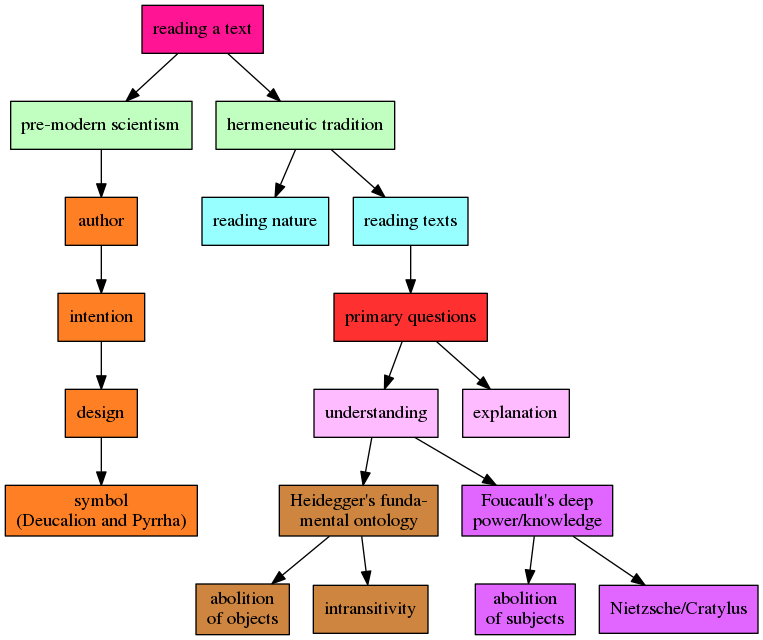
\includegraphics[scale=.32]{./subob.png}
\end{figure}
\end{frame}

\begin{frame}
  \frametitle{Hermeneutics of Trust}
  For Gadamer, a hermeneutics of suspicion is always derivative of a
  hermeneutics of trust (the contrast between the two is due to Paul
  Ricoeur, who wrote about this after Gadamer published \emph{Truth
    and Method}). Gadamer says, ``only when this assumption proves
  mistaken [the assumption that the text has integrity]---i.e.\ the
  text is not intelligible---do we begin to suspect the text'' (294).
  Understanding is like speaking your native language: it is natural,
  constitutive of being. Misunderstanding is derivative and
  artificial, such as when someone speaks to you in a foreign language
  that you do not understand.
  \begin{quote}
    It is only when the attempt to accept what is said as true fails
    that we try to ``understand'' the text, psychologically or
    historically, as another's opinion (294)
  \end{quote}
\end{frame}

\begin{frame}
  \frametitle{Hermeneutics of Suspicion}
  According to Ricoeur, the three purveyors of a hermeneutics of
  suspicion are:
  \begin{itemize}
  \item Friedrich Nietzsche
  \item Karl Marx
  \item Sigmund Freud
  \end{itemize}
Their trust counterparts are Rudolf Bultmann and Hans-Georg Gadamer
(and to some degree Ricoeur himself). 
\end{frame}

\begin{frame}
  \frametitle{Hermeneutic Circle}
  The hermeneutic circle is opposed to foundationalism. Examples are:
  \begin{itemize}
  \item the parts are determinative of the interpretation of the whole
    and vice versa
  \item the artist makes art; art defines and shapes the artist
  \item irreducibility does not imply independence
  \item interpretation presupposes understanding; understanding
    presupposes interpretation
  \end{itemize}
\end{frame}

\begin{frame}
  \frametitle{Structuralism}
\begin{figure}[h]
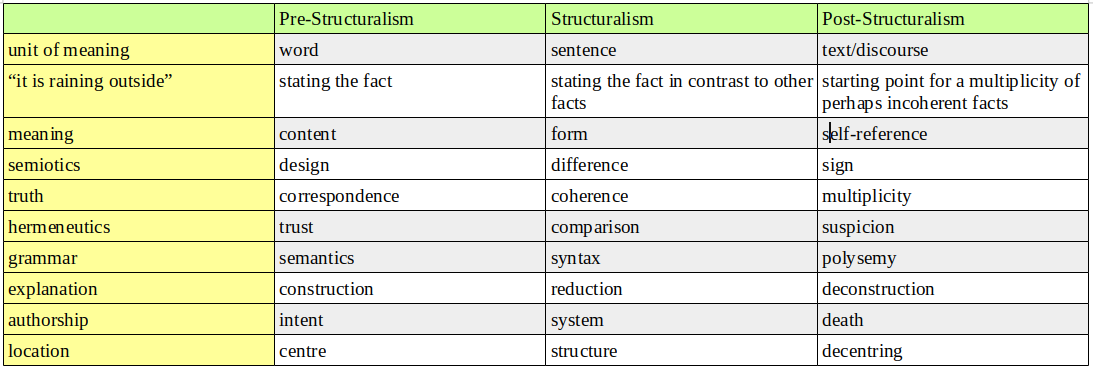
\includegraphics[scale=.3]{./structable.png}
\end{figure}
\end{frame}

\begin{frame}
  \frametitle{Philosophical Predecessors}
  Charles Taylor's critique has the following flavours:
  \begin{itemize}
  \item Aristotelian
    \begin{itemize}
    \item importance of upbringing and habits
    \item importance of making the parts fit the whole
    \item rational/emotional/social skills over rules
    \end{itemize}
  \item Narritivist (the importance of story)
  \item Hermeneutical (the importance of language and interpretation)
  \end{itemize}
\end{frame}

\begin{frame}
  \frametitle{The Expanding Circle}
Here is the expanding circle of Taylor's opponents:
\begin{itemize}
\item Utilitarianism
\item Existentialism
\item Nietzsche's Drive Psychology
\end{itemize}
\end{frame}

\begin{frame}
  \frametitle{Frankfurt's Second-Order Desires}
  \begin{itemize}
  \item first-order and second-order desires
  \item qualitative and quantitative evaluation of desires
  \item weak and strong evaluation (the defining feature for strong
    evaluation is to have a qualitative distinction of the worth of
    the motivations)
  \end{itemize}
Utilitarianism fails on two counts:
\begin{enumerate}
\item weak evaluation is not reducible to calculation
\item moral evaluation is not reducible to weak evaluation
\end{enumerate}
\end{frame}

\begin{frame}
  \frametitle{Criteria for Distinction}
  \begin{description}
  \item[contingency] strong evaluation dilemmas cannot be resolved by appeal to contingencies
  \item[contrast] strong evaluation proceeds on the basis of
    contrasts (courage is meaningless without cowardice and vice
    versa)
  \end{description}
\end{frame}

\begin{frame}
  \frametitle{The Problem with Second-Order Desires}
\begin{itemize}
\item the practical vs the moral approach to raising children (Taylor:
  ``deflated descriptions appear a wicked travesty, a shameless
  avoidance of moral reality,'' page 37)
\item consider a law that makes something morally repugnant
  (abortion, drug consumption, corruption, sex with children) more
  legal and less frequent $\longrightarrow$ would you assent to it?
\item are the moral notions at the basis of strong evaluation only
  a front to legitimize moral/social/economic pressure on others?
  (Mandeville)
\item the drug that allows you to eat cake and be healthy as well
  (deflated descriptions vs moral reality)
\item CT resolves this later by appealing to re-evaluation
\end{itemize}
\end{frame}

\begin{frame}
  \frametitle{J.S. Mill's Defence}
  Charles Taylor: ``honour, dignity, integrity are \emph{simply}
  other pleasurable states to which we give \emph{high-sounding}
  names'' (23). Why does reducibility in principle imply undue
  simplicity? Why is the ``simple weigher'' inferior to the
  ``strong evaluator''? Monism can be maintained even in the face
  of certain kinds of emergence (dialectical materialism).
  \begin{block}{Charles Taylor}
    thus the strong evaluator has articulacy and depth which the
    simple weigher lacks
  \end{block}
Really? Isn't it the monist who makes progress? Perhaps the monist
does not succeed with the reduction, but many productive (rather
than successful) scientific programs originate in a desire to
perform a reduction (alchemy). 
\end{frame}

\begin{frame}
  \frametitle{The Importance of Articulation}
  First-order choices are inarticulable. Second-order choices flow
  from the use of language and articulated coherence. Note the
  following analogy:
  \begin{itemize}
  \item Descartes' \textsc{je pense} solves an epistemological
    problem (skepticism); as a consequence, we perceive ourselves
    primarily and dominantly as thinking beings
  \item Taylor's \textsc{je parle} solves an ethical problem (what
    characterizes moral responsibility); as a consequence, we
    perceive ourselves primarily and dominantly as
    talking/interpreting/story-telling beings
  \end{itemize}
The story of my great-grandparents. 
\end{frame}

\begin{frame}
  \frametitle{Responsibility and Radical Choice}
  The problem with radical choice (Free French, Nepal) is that it
  solves the dilemma by rendering the force of the losing side
  inoperative (this is a problem that Bernard Williams has
  addressed with respect to utilitarianism and Kantian moral
  theory in articles such as ``Consequentialism and Integrity''
  and ``Ethical Consistency'' -- see his concept of ``regret'').

\bigskip

This is the core claim: agents of radical choice are simple
weighers. Taylor wasn't after the utilitarians, he was after the
existentialists, undermining their position by putting them in the
same boat as the utilitarians. The Meursault/Rieux incoherence
problem and what is the object of moral evaluation (in Taylor's
case: the way in which an agent successfully articulates coherence
in their life; in the existentialist's case: the way in which an
agent accepts the human condition).
\end{frame}

\begin{frame}
  \frametitle{Identity}
  \begin{block}{Charles Taylor}
    This is what is impossible in the theory of radical choice.
    The agent of radical choice would at the moment of choice have
    \emph{ex hypothesi} no horizon of evaluation. He would be utterly
    without identity. He would be a kind of extensionless point, a
    pure leap into the void. But such a thing is an impossibility,
    or rather could only be the description of the most terrible
    mental alienation. The subject of radical choice is another
    avatar of that recurrent figure which our civilization aspires
    to realize, the disembodied ego, the subject who can objectify
    all being, including his own, and choose in radical freedom.
    But this promised total self-possession would in fact be the
    most total self-loss. (35)
  \end{block}
\end{frame}

\begin{frame}
  \frametitle{Where Does the Buck Stop?}
Where does the buck stop? Not at radical choice (this would be a
sort of foundationalism), but at articulations (hermeneutic
circle). At the core are not calculations, but interpretations.
There is a hermeneutic circle from self-interpretations that are
constitutive of experience to evaluations of these
self-interpretations. Radical re-evaluation: Quine's web of
beliefs and Neurath's boat.  
\end{frame}

% \begin{frame}
%   \frametitle{iClicker Question}
% Choose from the following options. This item will be graded.
% \begin{block}{iClicker Question}
% [5902] What character of the future does Nietzsche describe in the
% Preface to Human All Too Human?
% \end{block}
% \begin{description}
% \item[A\hspace{.2in}$\blacktriangleright$] the bourgeois
% \item[B\hspace{.2in}$\blacktriangleright$] the free spirit
% \item[C\hspace{.2in}$\blacktriangleright$] the superman
% \item[D\hspace{.2in}$\blacktriangleright$] the nationalist antisemite
% \end{description}
% \end{frame}

% \begin{frame}
%   \frametitle{iClicker Question}
% Choose from the following options. This item will be graded.
% \begin{block}{iClicker Question}
% [5055] According to Nietzsche, to hold a person morally accountable is {\ldots}
% \end{block}
% \begin{description}
% \item[A\hspace{.2in}$\blacktriangleright$] {\ldots} a requirement of morality
% \item[B\hspace{.2in}$\blacktriangleright$] {\ldots} a feature of ethics to be defended at all costs
% \item[C\hspace{.2in}$\blacktriangleright$] {\ldots} an error with a historical explanation
% \item[D\hspace{.2in}$\blacktriangleright$] {\ldots} a necessity for happiness
% \end{description}
% \end{frame}

\begin{frame}
  \frametitle{Human, All Too Human: Preface}
  The free spirit
  \begin{itemize}
  \item revalues all values
  \item is more suspicious than trusting
  \item lives experimentally
  \item emerges from convalescence
  \item is master over his/her virtues
  \item embraces perspective and its injustice
  \end{itemize}
\end{frame}

\begin{frame}
  \frametitle{Human, All Too Human}
  Metaphyiscal philosophy vs historical philosophy (1, 1). Chemistry of
  concepts: how can something originate in its opposite? (Campari and
  cochineal beetles.) In 1,17 Nietzsche contrasts the metaphysical
  mode of explanation with physical and historical explanations.
  \begin{block}{Human All Too Human 1, 2}
    Philosophers involuntarily think of `man' as an aeterna veritas,
    as something that remains constant in the midst of all flux, as a
    sure measure of things.
  \end{block}
\end{frame}

\begin{frame}
  \frametitle{Human, All Too Human}
  Compare Kant and Nietzsche.
  \begin{quote}
    Two things fill the soul with awe and wonder: the starry heaven
    above, and the moral law within. (Kant)
  \end{quote}
  \begin{quote}
    For astrology believes that the firmament moves round the destiny
    of man; the moral man, however, takes it for granted that what he
    has essentially at heart must also be the essence and heart of
    things. (Nietzsche)
  \end{quote}
\end{frame}

\begin{frame}
  \frametitle{Human, All Too Human}
  Nietzsche's error theory of free will.
  \begin{block}{Human, All Too Human 2, 39}
    It is discovered that even this nature cannot be responsible,
    inasmuch as it is an absolutely necessary consequence concreted
    out of the elements and influences of past and present things,
    that man, therefore, cannot be made responsible for anything,
    neither for his nature, nor his motives, nor his actions, nor his
    effects. It has therewith come to be recognised that the history
    of moral valuations is at the same time the history of an error,
    the error of responsibility, which is based upon the error of the
    freedom of will.
  \end{block}
\end{frame}

\begin{frame}
  \frametitle{Human, All Too Human}
  Nietzsche's error theory of free will.
  \begin{block}{Human, All Too Human 2, 39}
    Nobody is responsible for his actions, nobody for his nature; to
    judge is identical with being unjust.
  \end{block}
\end{frame}

\begin{frame}
  \frametitle{Human, All Too Human}
  The evolution of good and evil. ``Good and bad is for a long time
  the same thing as noble and base'' (2, 45). Pity and benevolence.
  Pity is the power of the pitied to injure the pitier. The malice of
  pity and benevolence are medicine to assure a person of being able
  to dispense small amounts of power.
  \begin{block}{Human, All Too Human 2, 53}
    The heart of sensitive man ever enunciates against his head the
    axiom: between moral action and intellectual insight there must
    absolutely be a necessary connection. It is unfortunately
    otherwise; for there is no eternal justice.
  \end{block}
\end{frame}

% \begin{frame}
%   \frametitle{iClicker Question}
% Choose from the following options. This item will be graded.
% \begin{block}{iClicker Question}
% [1918] Which two Nietzsches are contrasted in Leiter's paper?
% \end{block}
% \begin{description}
% \item[A\hspace{.2in}$\blacktriangleright$] the \emph{Humean} and the \emph{Therapeutic} Nietzsche
% \item[B\hspace{.2in}$\blacktriangleright$] the \emph{German} and the \emph{Mediterranean} Nietzsche
% \item[C\hspace{.2in}$\blacktriangleright$] Nietzsche the \emph{atheist} and Nietzsche the \emph{agnostic}
% \item[D\hspace{.2in}$\blacktriangleright$] the \emph{Kantian} and the \emph{Utilitarian} Nietzsche
% \end{description}
% \end{frame}

% \begin{frame}
%   \frametitle{iClicker Question}
% Choose from the following options. This item will be graded.
% \begin{block}{iClicker Question}
% [6905] What about a person, according to Leiter's interpretation of Nietzsche, is psychologically determined?
% \end{block}
% \begin{description}
% \item[A\hspace{.2in}$\blacktriangleright$] moment of death
% \item[B\hspace{.2in}$\blacktriangleright$] type
% \item[C\hspace{.2in}$\blacktriangleright$] physiology
% \item[D\hspace{.2in}$\blacktriangleright$] token
% \end{description}
% \end{frame}

\begin{frame}
  \frametitle{Nietzsche's Naturalistic Moral Psychology}
  What is naturalism?
  \begin{enumerate}
  \item your inquiry is continuous with the methods of science
  \item you deny super-natural entities (because they play no
    explanatory role in science)
  \item you are skeptical about free will 
  \end{enumerate}
\end{frame}

\begin{frame}
  \frametitle{Nietzsche's Naturalistic Moral Psychology}
  The following offer a general theory of human nature, a
  (deterministic) Newtonian theory of psychology:
  \begin{itemize}
  \item David Hume (impressions and ideas)
  \item Karl Marx (dialectical materialism)
  \item Sigmund Freud (psychoanalysis)
  \end{itemize}
\end{frame}

\begin{frame}
  \frametitle{Nietzsche's Naturalistic Moral Psychology}
Nietzsche, in the tradition of Hume, offers a speculative psychology
since science was not advanced enough.
  \begin{block}{  Brian Leiter's \emph{doctrine of types}}
    Each person has a more-or-less fixed psycho-physical constitution,
    which defines him as a particular \emph{type} of person.
  \end{block}
\end{frame}

\end{document}
